%%%%%%%%%%%%%%%%%%%%%%%%%%%%%%%%%%%%%%%%%%%%%%%%%%%%%%%
% A template for Wiley article submissions.
% Developed by Overleaf. 
%
% Please note that whilst this template provides a 
% preview of the typeset manuscript for submission, it 
% will not necessarily be the final publication layout.
%
% Usage notes:
% The "blind" option will make anonymous all author, affiliation, correspondence and funding information.
% Use "num-refs" option for numerical citation and references style.
% Use "alpha-refs" option for author-year citation and references style.

\documentclass[alpha-refs]{wiley-article}
% \documentclass[blind,num-refs]{wiley-article}

% Add additional packages here if required
\usepackage{siunitx}
\usepackage{lineno}

% Update article type if known
\papertype{Original Article}
% Include section in journal if known, otherwise delete
\paperfield{Pest Management Science}

\title{Attract and kill: Spinosad containing spheres to control onion maggot (\textit{Delia antiqua})}

% List abbreviations here, if any. Please note that it is preferred that abbreviations be defined at the first instance they appear in the text, rather than creating an abbreviations list.
%\abbrevs{ABC, a black cat; DEF, doesn't ever fret; GHI, goes home immediately.}

% Include full author names and degrees, when required by the journal.
% Use the \authfn to add symbols for additional footnotes and present addresses, if any. Usually start with 1 for notes about author contributions; then continuing with 2 etc if any author has a different present address.
\author[1\authfn{1}]{Denis S. Willett}
\author[1\authfn{1}]{Camila C. Filgueiras}
\author[1]{Jan P. Nyrop}
\author[1]{Brian A. Nault}

\contrib[\authfn{1}]{Equally contributing authors.}

% Include full affiliation details for all authors
\affil[1]{Department of Entomology, Cornell AgriTech, Cornell University, Geneva, NY, 14456, USA}

\corraddress{Denis S. Willett, 15 Castle Creek Drive, Geneva, NY 14456}
\corremail{deniswillett@cornell.edu}


% Include the name of the author that should appear in the running header
\runningauthor{Willett et al.}

\begin{document}

\maketitle

\begin{abstract}

BACKGROUND: Onion maggot (\textit{Delia antiqua}) is a pest of onions worldwide. Current means of managing this pest rely heavily on prophylatic insecticide treatments at planting. These options may not be viable in organic production systems or situations where insecticide-resistant populations occur. Here we explore the efficacy of an attract and kill strategy for control of \textit{D. antiqua} evaluating the ability of attractive, spinosad containing spheres to kill adult \textit{D. antiqua} and reduce crop losses. 

RESULTS: Spinosad containing spheres were able to consistently kill \textit{D. antiqua} adults over the course of the field season (mortality range: between 49\% and 59\% on average). Pairing spinosad spheres with Delia Lure increased efficacy by 72\% compared with the spheres alone. Performance of this attract and kill strategy also can reduce damage by \textit{D. antiqua}  larvae in the field, but it did not achieve a level of control comparable to the level provided by a conventional insecticide treatment. 

CONCLUSION: Implementation of this attract and kill strategy could be a valuable tool in situations where conventional pesticides are either not available or desired, where additional control techniques are needed, or to provide a season-long option for control of \textit{D. antiqua} populations.

% Please include a maximum of seven keywords
\keywords{Onion Maggot, \textit{Delia antiqua}, attraction, sticky-trap, attract-and-kill, lure, onion management}
\end{abstract}

\linenumbers
\section{Introduction}

Allium crops worldwide suffer attack from onion maggot (\textit{Delia antiqua} Meigen).  Present in the Americas, Europe and Asia, \textit{Delia antiqua} is well established in most temperate onion growing regions and causes crop losses of up to 100 percent on onions (\textit{Allium cepa} L) if left unmanaged \citep{nault2006performance, nault2006onion}.  Other allium crops including garlic (\textit{Allium sativum} L.), scallions (\textit{Allium fistulosum} L.), and chives (\textit{Allium schoenoprasum} L.) are similarly susceptible \citep{ellis1979factors,ning2017predicting,nault2007ecology}.  Commercial onion production has relied upon intensive management of this pest, but losses continue to occur in places where crop rotation is not used and insecticide-resistant populations are present \citep{martinson1988dispersal, nault2006onion}.  

The lifecycle of \textit{Delia antiqua} plays a large role in its severity as an onion pest.  In the northern United States, three generations per year are common \citep{eckenrode1975population, hoepting2004insecticide}. In New York, \textit{D. antiqua} overwinters as a pupa and adults emerge in late April to early May and peak in late May to early June. The next generation begins to emerge in late June to early July and peaks in mid to late July, while the last generation adults begin to emerge in late July to early August and peak in mid to late August \citep{nault2011delaying}. While adults can be captured in fields using sticky cards, the larvae cause devastating damage by feeding on plant roots and onion bulbs \citep{nault2006onion, nault2006performance}. Feeding by \textit{D. antiqua} larvae early in the season can kill seedlings and damaged plants can become more susceptible to infection by pathogen and attack by subsequent generations \citep{eckenrode1986impact,nault2006performance}.  Feeding by \textit{D. antiqua} larvae, even if it does not completely kill the onion can cause sufficient damage to prevent sale of the bulb.   

Management of \textit{D. antiqua} has relied on prophylactic insecticide applications at planting \citep{nault2006performance}. A variety of organophosphate and carbamate insecticides have been used and discontinued \citep{nault2006performance}. Chlorpyrifos (Lorsban Advanced) is still commonly used as a drench treatment in combination with either cyromazine seed treatment (Trigard) \citep{nault2006performance,nault2006onion} or the seed treatment package containing thiamethoxam, spinosad and several fungicides (FarMore FI500); although some growers rely exclusively on FarMore FI500 to manage \textit{D. antiqua}. Cultural practices such as crop rotation, removal of damaged cull and volunteer onions, and delayed planting are also effective \textit{D. antiqua} management tactics \citep{martinson1988dispersal,finch1985influence,nault2011delaying} but they are not typically adopted by large-scale commercial growers.   

Recent advancements in monitoring \textit{D. antiqua} populations have created the possibility of a new control strategy. \textit{Delia antiqua} adults respond to and are attracted by visual and chemical cues \citep{harris1988host,harris1983color,thomingdeveloping,otto2000development}. Visually, \textit{D. antiqua} adults tend to prefer large white spheres, while chemically they respond strongly to chemical constituents of decomposing onion. In particular, two components of decomposing onion, 2-phenyl-ethanol and n-valeric acid, are attractive and have been formulated into attractive lures \citep{ishikawa1984mixture,ishikawa1987controlled,kuhar2006field}. Combining the white spheres with a chemically attractive lure, Delia Lure (AgBio, Westminster, CO), approximately doubled \textit{D. antiqua} adult trap catch \citep{willett2019}. Adding an insecticide to these attractive spheres could be an effective attract and kill solution for controlling \textit{D. antiqua}.

Attract and kill strategies rely on pairing an attractive component, usually involving a semiochemical and/or visual component, with a killing component whether through mechanical or chemical means \citep{gregg2018advances}.  Attract and kill strategies can be more specific and environmentally friendly and have previously contributed to integrated pest management of flies and moths \citep{gregg2018advances}.  Of particular interest and inspiration for this work, red insecticide-treated spheres were developed as an attract and kill solution for control of apple maggot (\textit{Rhagoletis pomonella} (Walsh)) in northeastern orchards \citep{bostanian2001attract,duan1995control}.  

Choice of the killing component in an attract and kill solution for use in an integrated pest management program is important. For working with \textit{D. antiqua} control, we elected to use spinosad as the toxicant. Spinosad is a naturally derived neurotoxic insecticide originally isolated from the soil-dwelling actinomycete \textit{Saccharopolyspora spinosa} \citep{racke2007reduced}. It has been approved for use on over 150 fruit and vegetable crops in the United States and is certified for use in organic production by the USDA National Organic Standards Board and Organic Materials Review Institute (OMRI) \citep{racke2007reduced,williams2003naturally}. In addition, spinosad has substantially lower non-target effects relative to conventional pesticides and a low residual toxicity \citep{williams2003naturally}. Because of its complementary nature to current conventional management of \textit{D. antiqua} and potential use in organic production systems, spinosad was included in the development of an attract and kill solution for \textit{D. antiqua}.

To develop an effective attract and kill solution to control \textit{D. antiqua}, we combined attractive white spheres developed in previous work \citep{willett2019} with a spinosad insecticide solution. We hypothesized that these spinosad-attractive spheres would kill \textit{D. antiqua} flies and significantly reduce maggot damage to onions in the field. This study was conducted over the course of three field seasons in upstate New York.

\section{Materials and Methods}

Field trials evaluating the efficacy of attract and kill strategies to manage \textit{D. antiqua} populations were conducted from 2006 to 2008 in commercial dry bulb onion fields on muck soils in upstate New York, USA.  Muck soils are high organic matter soils formed from old lake beds.  Trials were conducted from May to September.  All field sites used in these trials had a history of continuous onion production, had historically relatively prominent \textit{D. antiqua} populations, and grower collaborators interested in improving management.  

\subsection{Population Monitoring}

Population monitoring of \textit{D. antiqua} adults was accomplished in 2006 by deploying white sticky cards in triplicate along onion field edges in each of six commercial onion fields.  Field edges have been identified as ideal locations for trapping adult fly populations, especially when borders abut woodlands \citep{werling2006spatial}.  Cards were collected weekly from May to September and the number of male and female adult flies counted.

\subsection{\textit{D. antiqua} Mortality}

Because white spheres are highly attractive to \textit{D. antiqua} adults, 1\%, 0.5\%, and 0\% (control) spinosad were added to paraffin and coated on 8.75cm diameter white plastic spheres to evaluate the ability of the spheres to cause \textit{D. antiqua} mortality. Additionally, the temporal efficacy of the spinosad solution was evaluated.

To do so, the ability of spinosad spheres to kill \textit{D. antiqua} flies was evaluated over the course of 2006 and 2007 field seasons by deploying a cohort of spheres containing spinosad at the beginning of the season (mid May) and recovering a subset of them on a monthly basis to evaluate weather exposure and dose effects.  Following initial deployment in mid May spheres were recovered in mid June, mid July, mid August, and mid September resulting in cohorts exposed to field conditions for 1 month, 2 months, 3 months, 4 months, respectively. Deployment in the field followed a randomized controlled block design with six replicates of the 12 treatments (3 spinosad levels x 4 periods of field exposure) across three field sites from 2006 to 2007.  Spheres were suspended from 30cm long stakes placed along the long side of the onion field at a spacing of 15.2m.  

Following recovery from the field, spheres were photographed to document degradation, then each one was immediately suspended in 25cm x 25cm x 50cm screen and plexiglass cages containing water in a petri dish. Ten male and ten female \textit{D. antiqua} flies were then introduced to each cage and mortality monitored every 24 hours for 72 hours. This trial was conducted for both spinosad containing and control spheres. 
 

\subsection{Field Damage}

To evaluate the efficacy of attract and kill techniques for reducing \textit{D. antiqua} larval damage, onions killed or damaged by \textit{D. antiqua} larvae were monitored throughout the field seasons of 2007 and 2008. Onion seed of \textit{Allium cepa} L. ’Arsenal’, an early yellow globe variety, was planted in late April with plants subjected to treatments in a randomized controlled block design with six replicates across three field sites.  Six treatment combinations were evaluated (i.e., insecticide-treated plants only [positive control], non-insecticide treated plants with spinosad containing white spheres only, non-insecticide treated plants with spinosad containing white spheres and Delia Lure, non-insecticide treated plants with white sticky cards only, non-insecticide treated plants with white sticky cards and Delia Lure, and non-insecticide treated plants only [negative control]).  Insecticide-treated plants were grown from seeds treated with the FarMore FI500 seed treatment package. This treatment was included in the experiment to be a positive control. Non-insecticide treated plants were grown from fungicide-only treated seeds (thiram [Thiram 42 S {@}188 mg a.i./ 100 g seed] and tebuconazole [Raxil 2.6 F @ 250 mg a.i. / 100 g seed]) and did not receive any attract and kill strategies. Spinosad spheres containing 0.5\% spinosad were deployed with and without attractive Delia Lures (AgBio, Westminster, CO) as an attract and kill solution. White sticky cards with and without attractive Delia Lure were also deployed. 

Each individual experimental plot was 8 rows by 9.1m  long separated from its nearest neighboring experimental plot by a minimum of 30.5m in any direction. Three weeks following planting, seedlings in the middle two rows were counted to obtain an initial stand count. Following initial stand count, plant loss due to damage by \textit{D. antiqua} larvae was evaluated on a weekly basis in the middle two rows until the end of season when a final stand count was taken (including all mortality factors). Plants killed by \textit{D. antiqua} were assessed visually, then confirmed by removing the plant and ascertaining presence of \textit{D. antiqua} larvae. When plants became too large to visually detect \textit{D. antiqua} damage, subsamples of plants were removed from the soil and bulbs inspected for \textit{D. antiqua} larvae and larval feeding damage. The overall percentage of cumulative \textit{D. antiqua} damaged plants for the season was determined. 

\subsection{Enhanced Formulation}

To enhance attractiveness, longevity, and performance of spinosad containing spheres, a new formulation of spinosad containing sphere was developed with 0.5\% spinosad, 5.0\% ammonium carbonate and 5.0\% casein hydrolysate to stabilize the paraffin and improve performance. The efficacy of this new formulation was compared with spheres containing just 0.5\% spinosad and no spinosad controls in field cage trials in 2008. Treatments were deployed in a randomized controlled block design with four replications and each individual plot consisted of four rows of onion each 3.7m (12ft)  long. All onion seeds including those in the untreated control were treated with fungicides: thiram (Thiram 42 S {@}188 mg a.i./ 100 g seed) and tebuconazole (Raxil 2.6 F @ 250 mg a.i. / 100 g seed). Seeds were planted in early May and each plot was caged (3.7m x 3.7m x 2m) using PVC pipe and screen mesh. One hundred fifty \textit{D. antiqua} flies with a 50:50 male to female ratio were released into each cage on the second of June and again nine days later on June 11th. As described above, initial and final stand counts were taken and plant damage due to \textit{D. antiqua} larvae evaluated on a weekly basis.  


\subsection{Analysis}

To evaluate population dynamics of \textit{D. antiqua} over time, a smoothing function consisting of a generalized additive model with cubic splines was fitted to the raw population numbers for visual display.  

To evaluate adult \textit{D. antiqua} mortality as a result of contact with spheres containing spinosad, linear models and analysis of variance were used.  Models were determined after consideration of all factor combinations (rate and exposure time for mortality trials and control strategy and presence of Delia Lure with date as a random effect for field trials) and interactions and selected based on residual diagnostics (conformance to assumptions of normality and homoscedasticity), goodness of fit tests, $R^2$ values, information criteria (AIC and BIC), leverage, and likelihood ratio tests. Main effects and means separations were evaluated using Tukey and Dunnett post-hoc tests at $P < 0.05$.  

Field damage and stand loss were evaluated using mixed effects linear and negative binomial models.  Best fit models were selected after consideration of data distributions, residual diagnostics, likelihood ration considerations, information criteria, and psuedo-$R^2$ values, root mean squared error and coefficient of variation of root mean squared error.  


\subsection{Data Management}

All data for the trials were entered into flat tabular (.csv) files.  All analysis on the raw data was conducted in R version 3.5.2 using RStudio as an IDE (with Vim keybindings) \citep{rcore2018,rstudio}.  The $tidyverse$, $car$, $lme4$, and $emmeans$ packages were used to facilitate analysis \citep{tidy, car, lme, emmeans}.  All code, including manuscript documentation, is available on GitHub (https://github.com/acetworld/onion-maggot-control).


\section{Results}

\paragraph{Population Monitoring}

Over the course of the 2006 field season when population surveys were conducted in upstate New York, \textit{D. antiqua} had three generations (Figure \ref{fig:figure1}).  The first population of adults peaked in June, the second in late July, and the third in August.  More males than females were collected on sticky cards, but both males and females followed roughly the same population cycles. 

\paragraph{\textit{Delia antiqua} Mortality}

White spheres containing spinosad caused significant mortality of \textit{D. antiqua} adults compared to controls (Figure \ref{fig:figure2}A).  Both spinosad rate (F =114.3, df=2, p \textless 0.001)  and exposure time (F = 4.7, df = 1, p = 0.03) in the field significantly explained approximately 62\% of the observed variation in adult \textit{D. antiqua} mortality ($R^2_{adj}$ = 0.62, p \textless 0.001).  Both rates of spinosad treated spheres caused approximately 47$\pm$4\% more \textit{D. antiqua} mortaliy than untreated controls (Figure \ref{fig:figure2}B).  Increasing rates of spinosad from 0.5\% to 1\% did not signifcantly increase \textit{D. antiqua} mortality (Figure \ref{fig:figure2}B).  

Increasing time spent in the field decreased efficacy of spinosad containing spheres (Figure \ref{fig:figure2}C).  For every month of exposure, mortality of \textit{D. antiqua} tended to decline 3$\pm$1\%.  After four months of exposure, and despite obvious degradation of the paraffin containing the spinosad (Figure \ref{fig:figure2}D), \textit{D. antiqua} mortality as a result of contacting spinosad containing spheres still remained above 45\% (Figure \ref{fig:figure2}C).  

\textit{D. antiqua} mortality as a result of contacting spinosad containing spheres was not constant over the 72 hours of monitoring in cages (Figure \ref{fig:figure3}).  For both spinosad rates, \textit{D. antiqua} mortality tended to peak at around 48 hours for spheres with one month exposure to field conditions (the June cohort).  After longer exposure to field conditions, \textit{D. antiqua} mortality tended to decline over the course of 72 hours.  

\paragraph{Field Damage}

Deployment of the attract and kill solution of spinosad containing spheres did influence cumulative onion damage in the field as a result of \textit{D. antiqua} larval feeding (Figure \ref{fig:figure4}A).  Cumulative damage as a result of \textit{D. antiqua} larval feeding was significantly explained by treatment solution ($\chi^2$ = 42.2, df = 3, p \textless 0.001), the presence of Delia Lure ($\chi^2$ = 10.0, df = 1, p = 0.001), and their interaction ($\chi^2$ = 21.4, df = 1 p \textless 0.001).  Cumulative damage due to feeding by \textit{D. antiqua} larvae over the course of the field season ranged from 0 in some control plots to 82 dead \textit{D. antiqua} plants in a few plots. This amounts to approximately 20-30\% losses of onion directly attributable feeding by \textit{D. antiqua} larvae.  All treatments were significantly worse than insecticide controls which had very low levels of \textit{D. antiqua} damage (Figure \ref{fig:figure4}A).  Pairing Delia Lure with spinosad containing spheres significantly reduced damage by \textit{D. antiqua} larvae by 72$\pm$10\% (p \textless 0.001) compared to spinosad spheres alone.  Pairing Delia Lure with sticky cards had the opposite effect (P = 0.002, Figure \ref{fig:figure4}A).

\paragraph{Enhanced Formulation}

Treatment (implementation of attract and kill strategies) significantly explained observed \textit{D. antiqua} damage in field cage trials with the enhanced formulation ($\chi^2$ = 23.9, df = 2, p \textless 0.001).  The enhanced formulation (spinosad +) containing 0.5\% spinosad, 5.0\% ammonium carbonate and 5.0\% casein hydrolysate did not perform significantly different (t = -1.9, df = 64, p = 0.13) than spinosad-only treatments with 0.5\% spinosad containing spheres (Figure \ref{fig:figure4}B).  Both treatments containing spinosad performed significantly better than the no insecticide controls (Spinosad: t = 4.9, df = 64, p \textless 0.0001; Spinosad +: t = 2.9, df = 64, p = 0.01, Figure \ref{fig:figure4}B).  


\begin{figure}[bt]
\centering
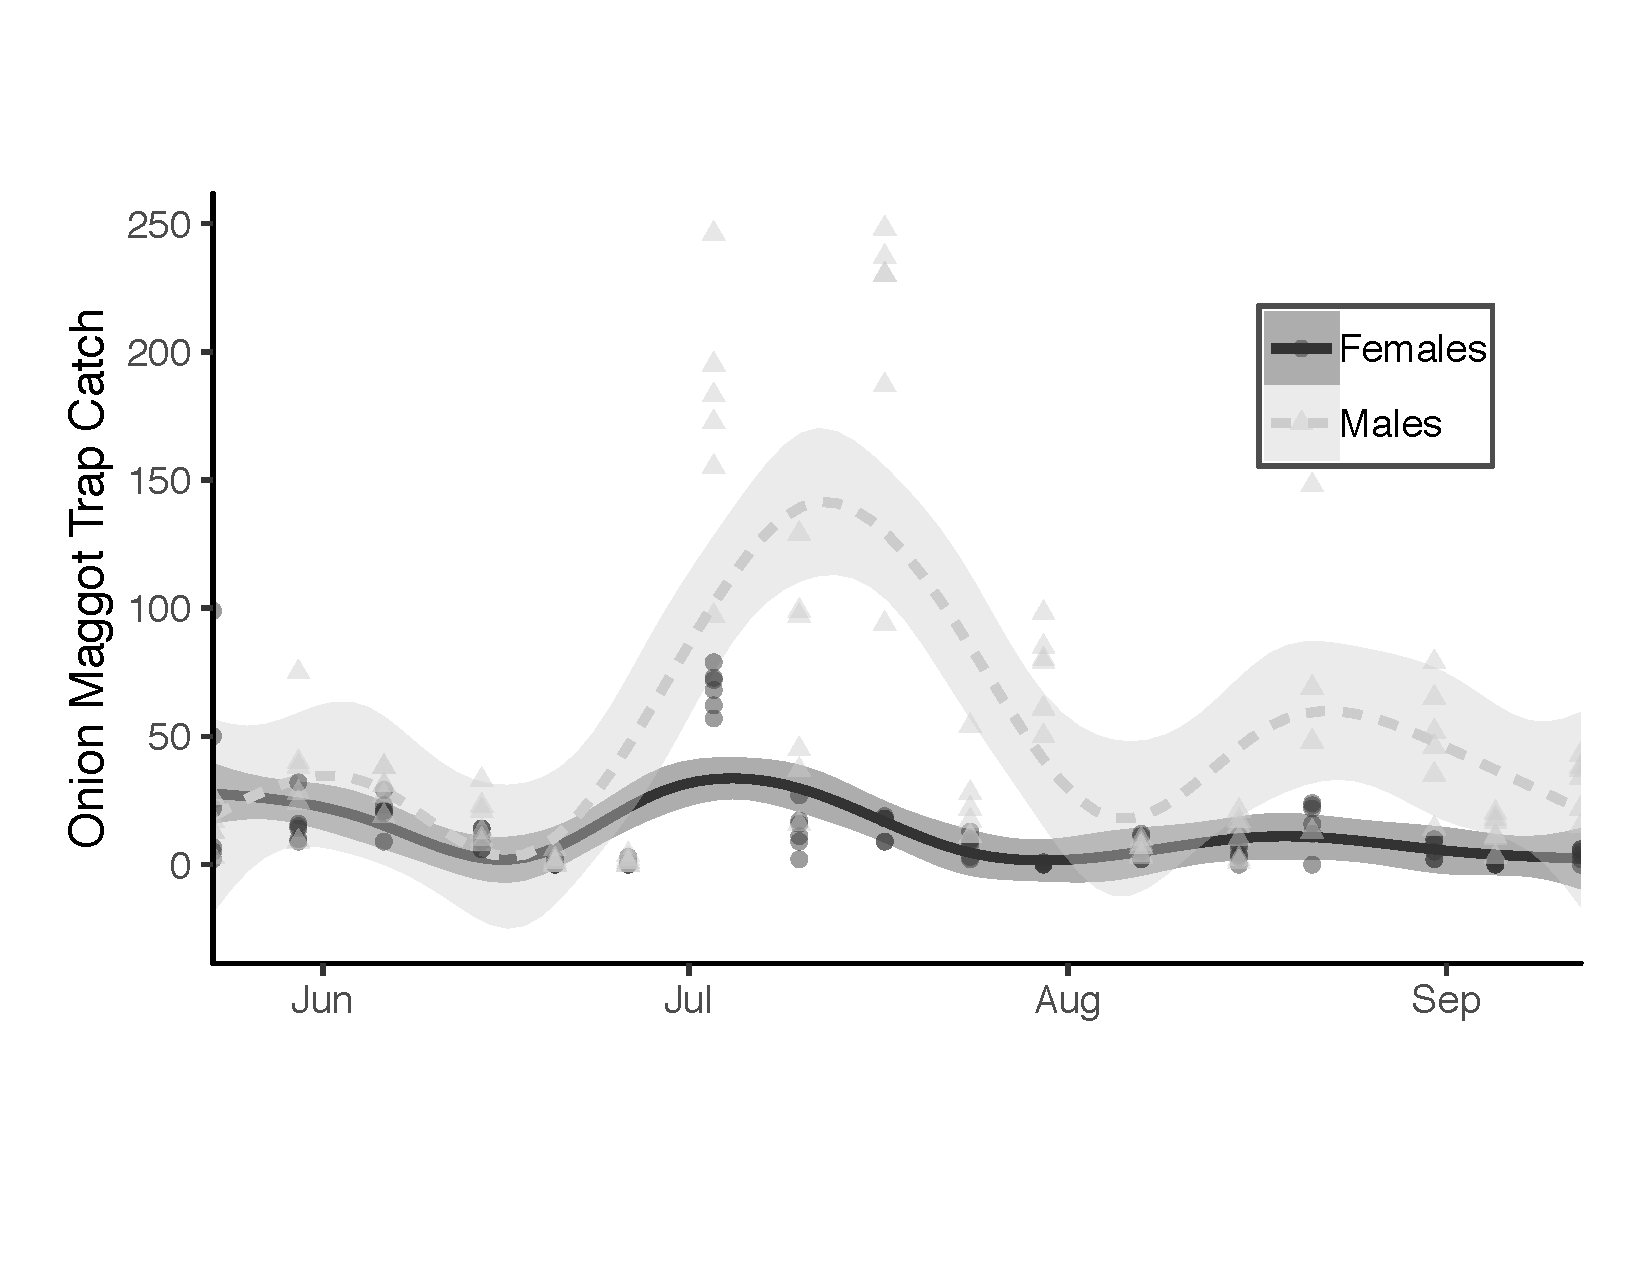
\includegraphics[width = 8cm]{figures/final-figures/figure-1.pdf}
\caption{Population dynamics of adult onion maggot (\textit{D. antiqua}) flies in upstate New York muck regions.  Points indicate observations of numbers of adult flies captured on sticky cards.  Lines and shaded regions indicate smoothed fits and 95\% confidence intervals respectively.  }
\label{fig:figure1}
\end{figure}

\begin{figure}[bt]
\centering
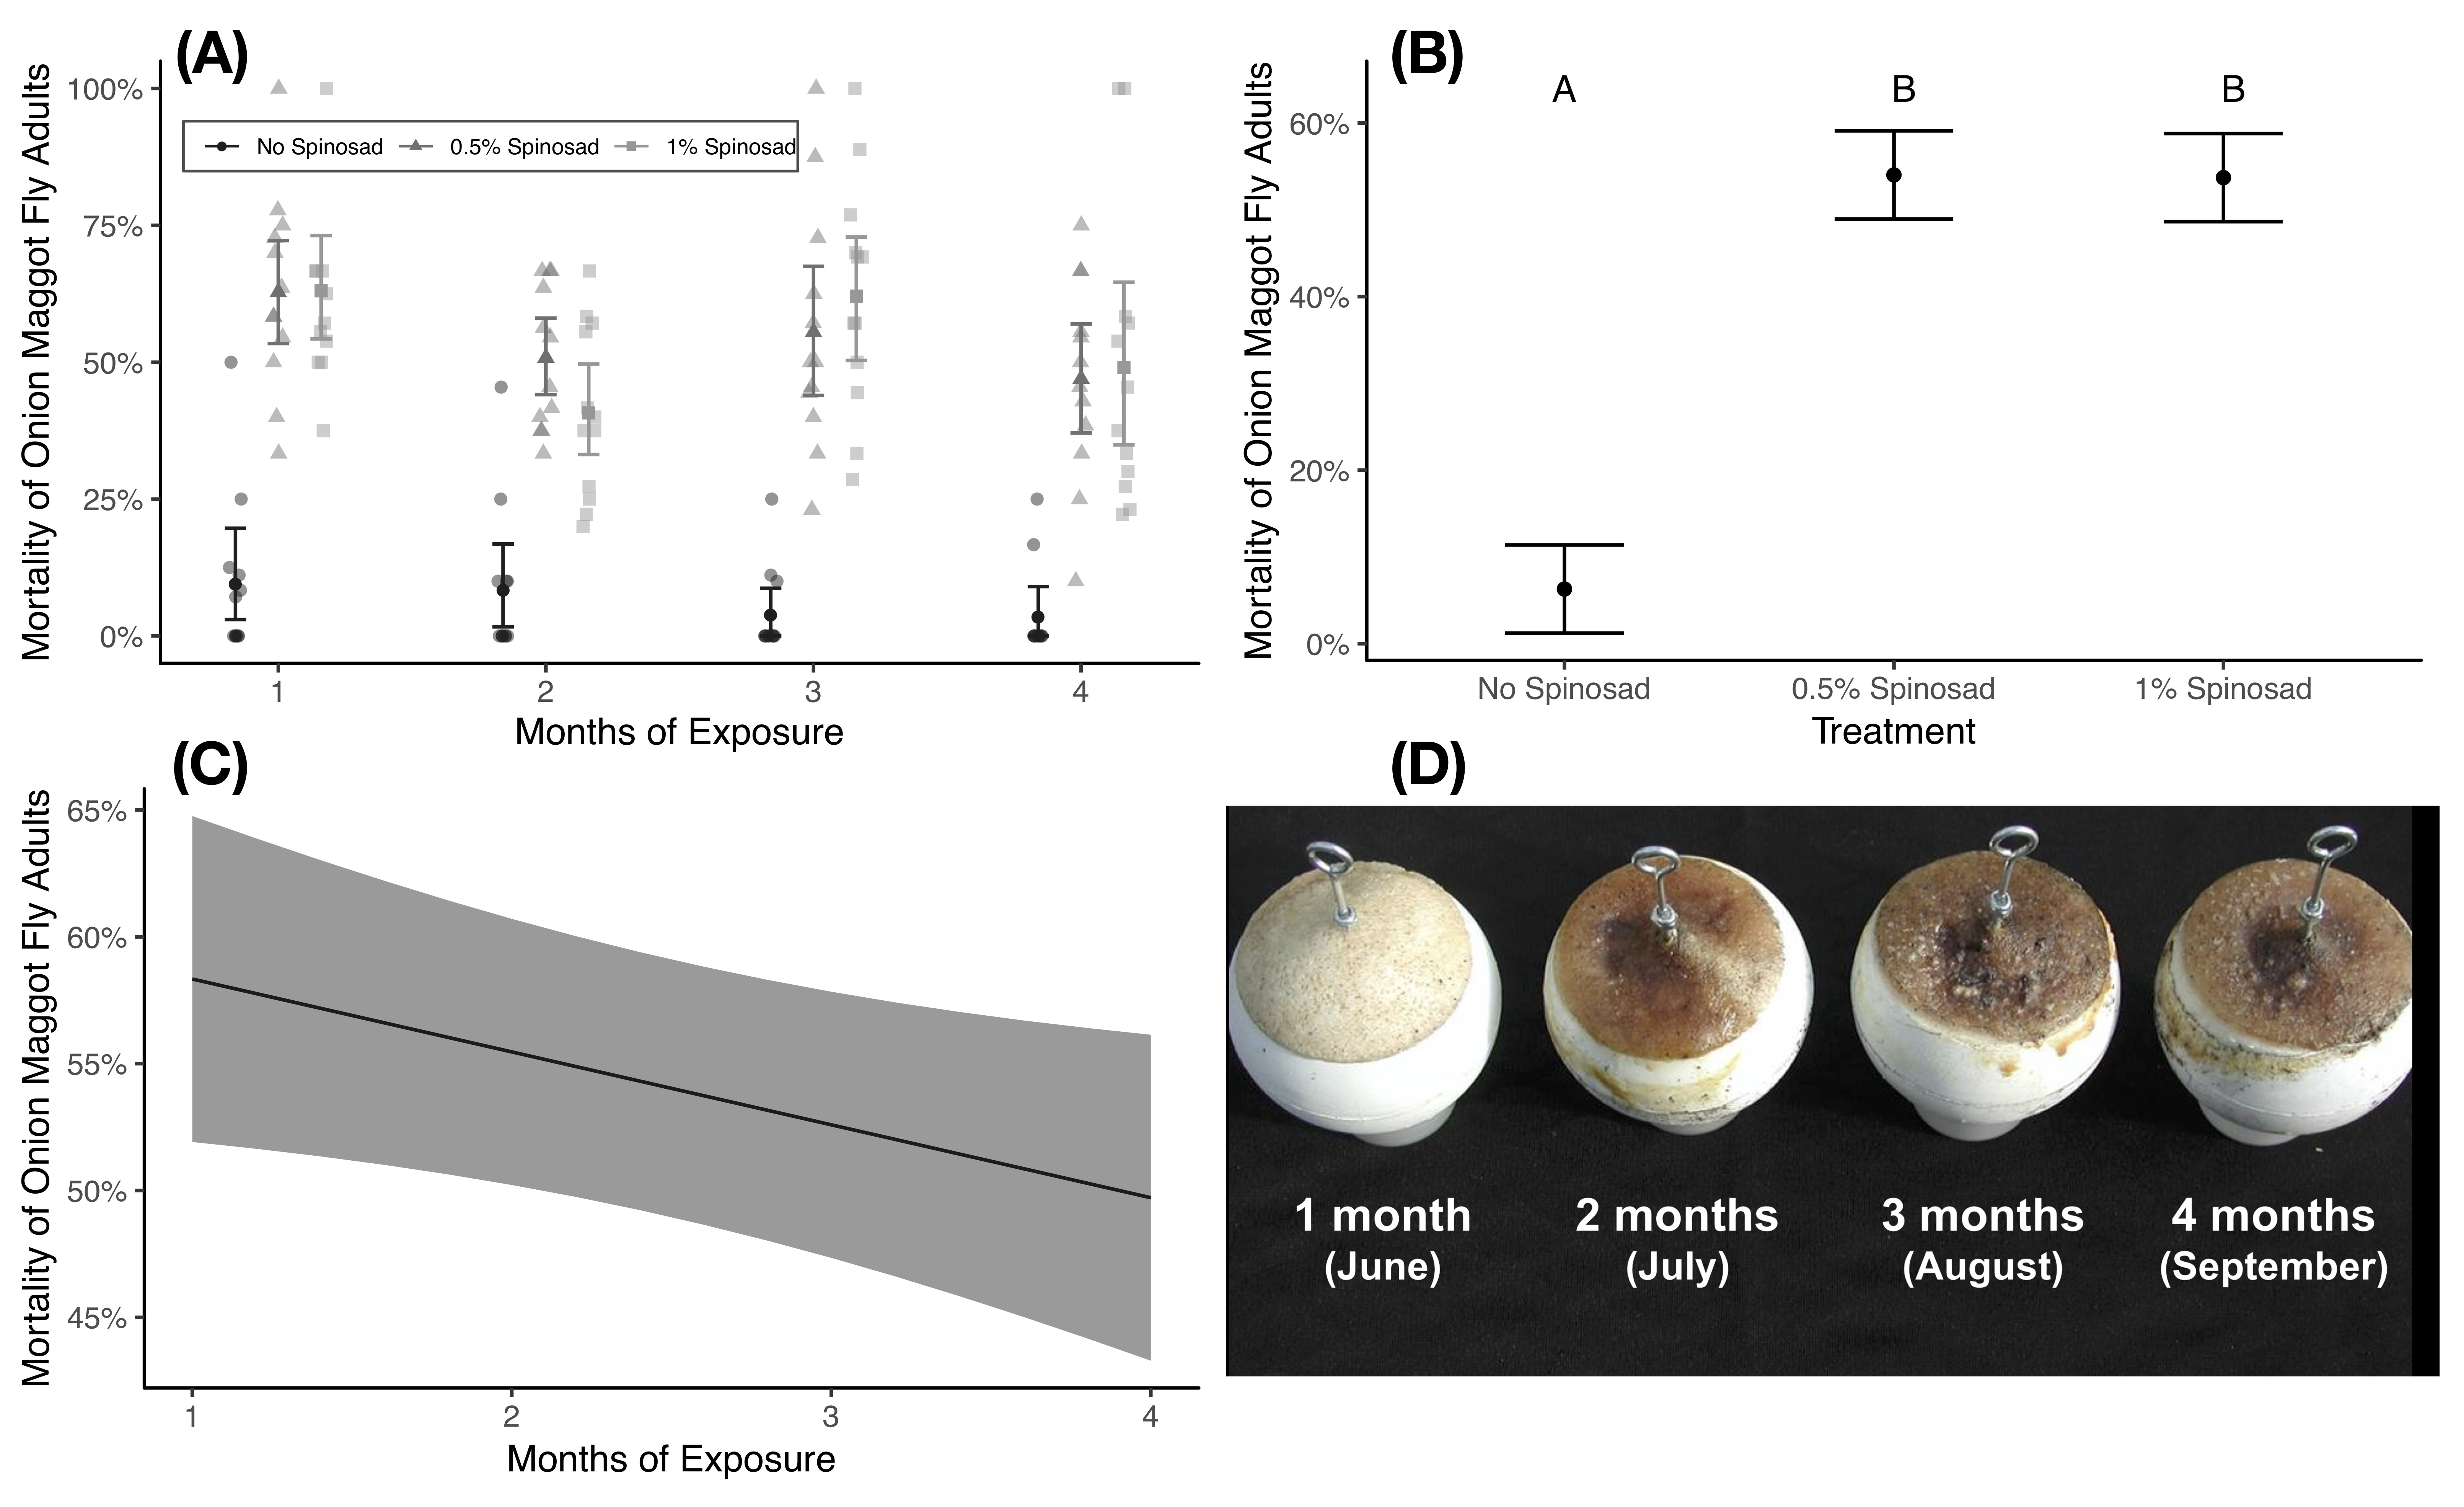
\includegraphics[width = 8cm]{figures/final-figures/figure-2.pdf}
\caption{Adult onion maggot (\textit{D. antiqua}) mortality in the presence of spinosad treated spheres.  (A) Raw data of effects of exposure time and spinosad rate on mortality of adult \textit{D. antiqua} flies.  Light points indicate individual observations.  Solid points and error bars denote mean and 95\% confidence intervals respectively.  (B) Main effects of spinosad rate on adult \textit{D. antiqua} mortality.  Points and error bars denote mean effect and 95\% confidence intervals respectively.  Different letters denote significant differences (p \textless 0.05).  (C) Main effect of exposure time on adult \textit{D. antiqua} mortality.  Line and shaded area denote effect and 95\% confidence region respectively.  (D) Photographs of spinosad treated spheres at increasing exposure time in field conditions.  Spheres were placed in the field on the 15th of May.  }
\label{fig:figure2}
\end{figure}


\begin{figure}[bt]
\centering
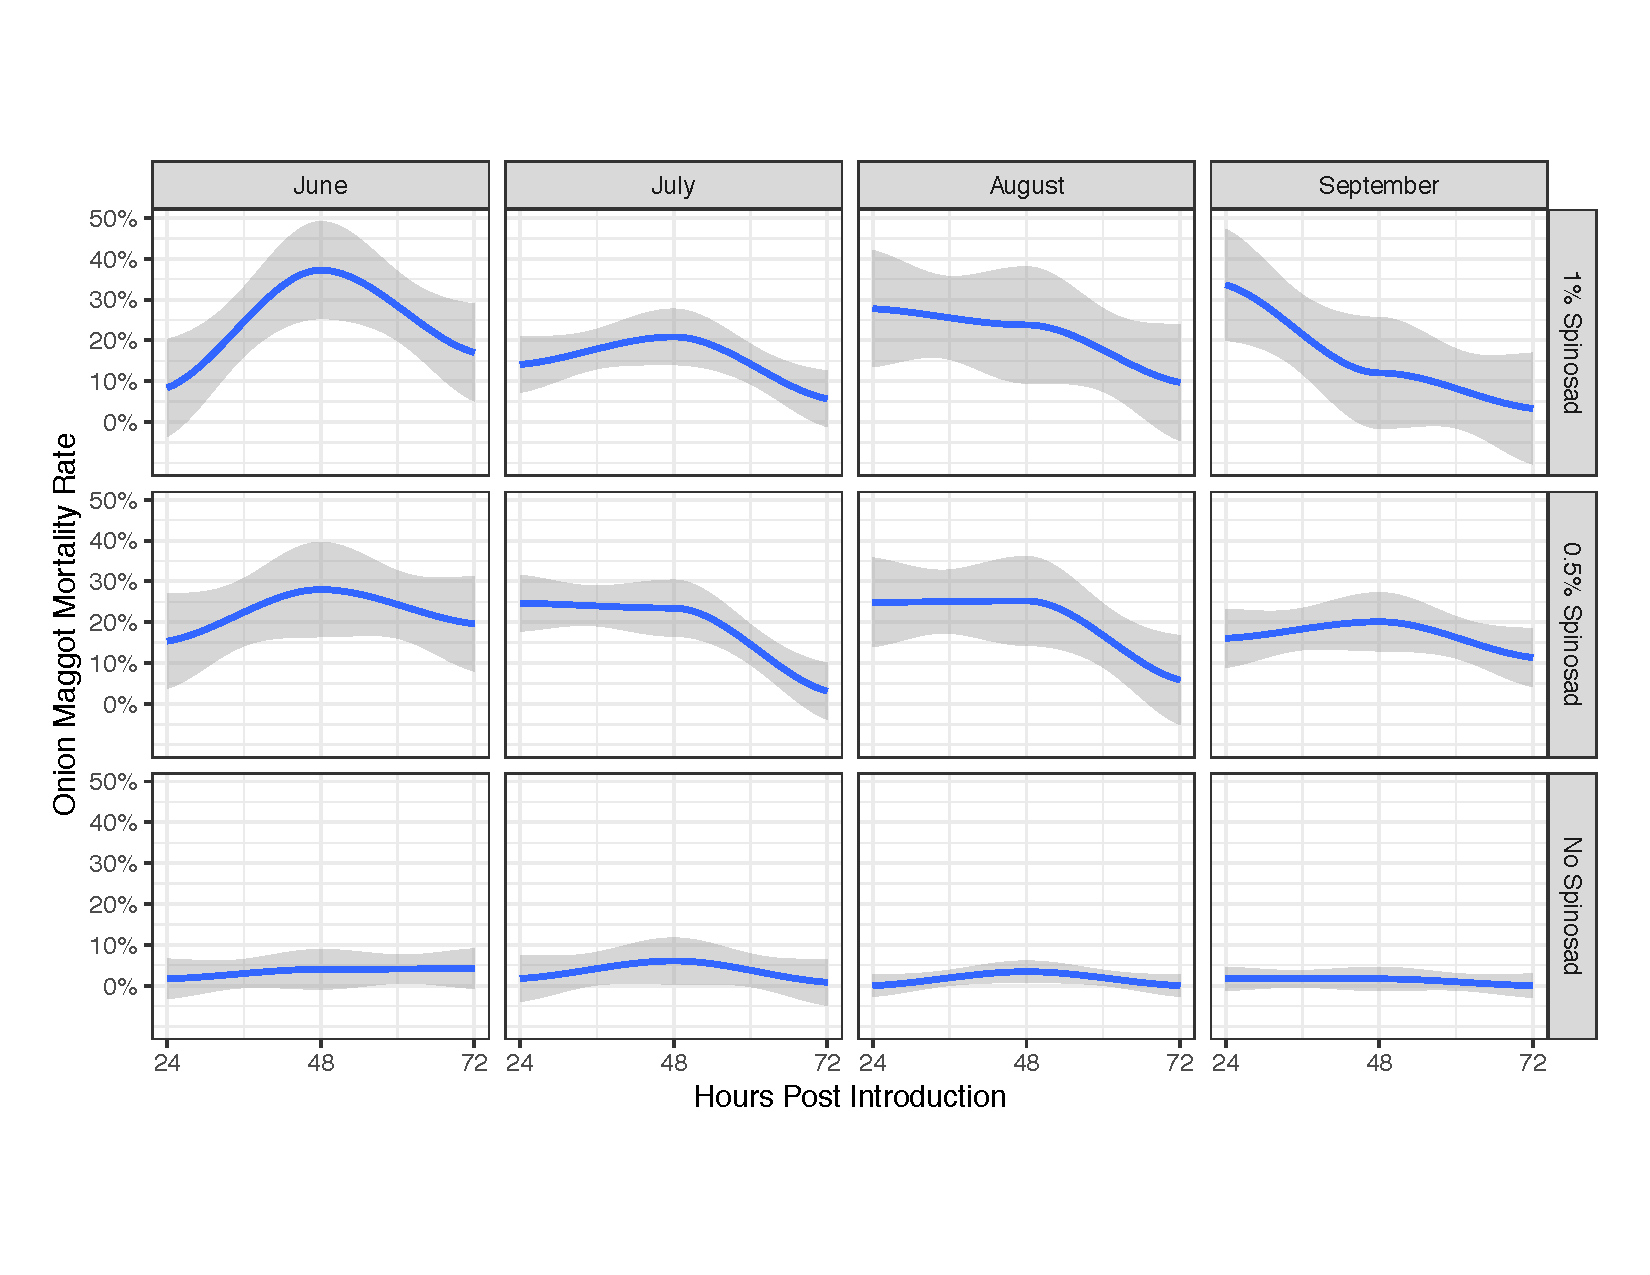
\includegraphics[width = 8cm]{figures/final-figures/figure-3.pdf}
\caption{Adult onion maggot (\textit{D. antiqua}) fly mortality following introduction to cages containing spinosad treated spheres.  Spheres were treated with differing rates of spinosad (rows) and exposed to field conditions for increasing amounts of time (column).  Lines and shaded regions indicate fitted smoothed (LOESS) mortality rates and 95\% confidence regions respectivel.  }
\label{fig:figure3}
\end{figure}


\begin{figure}[bt]
\centering
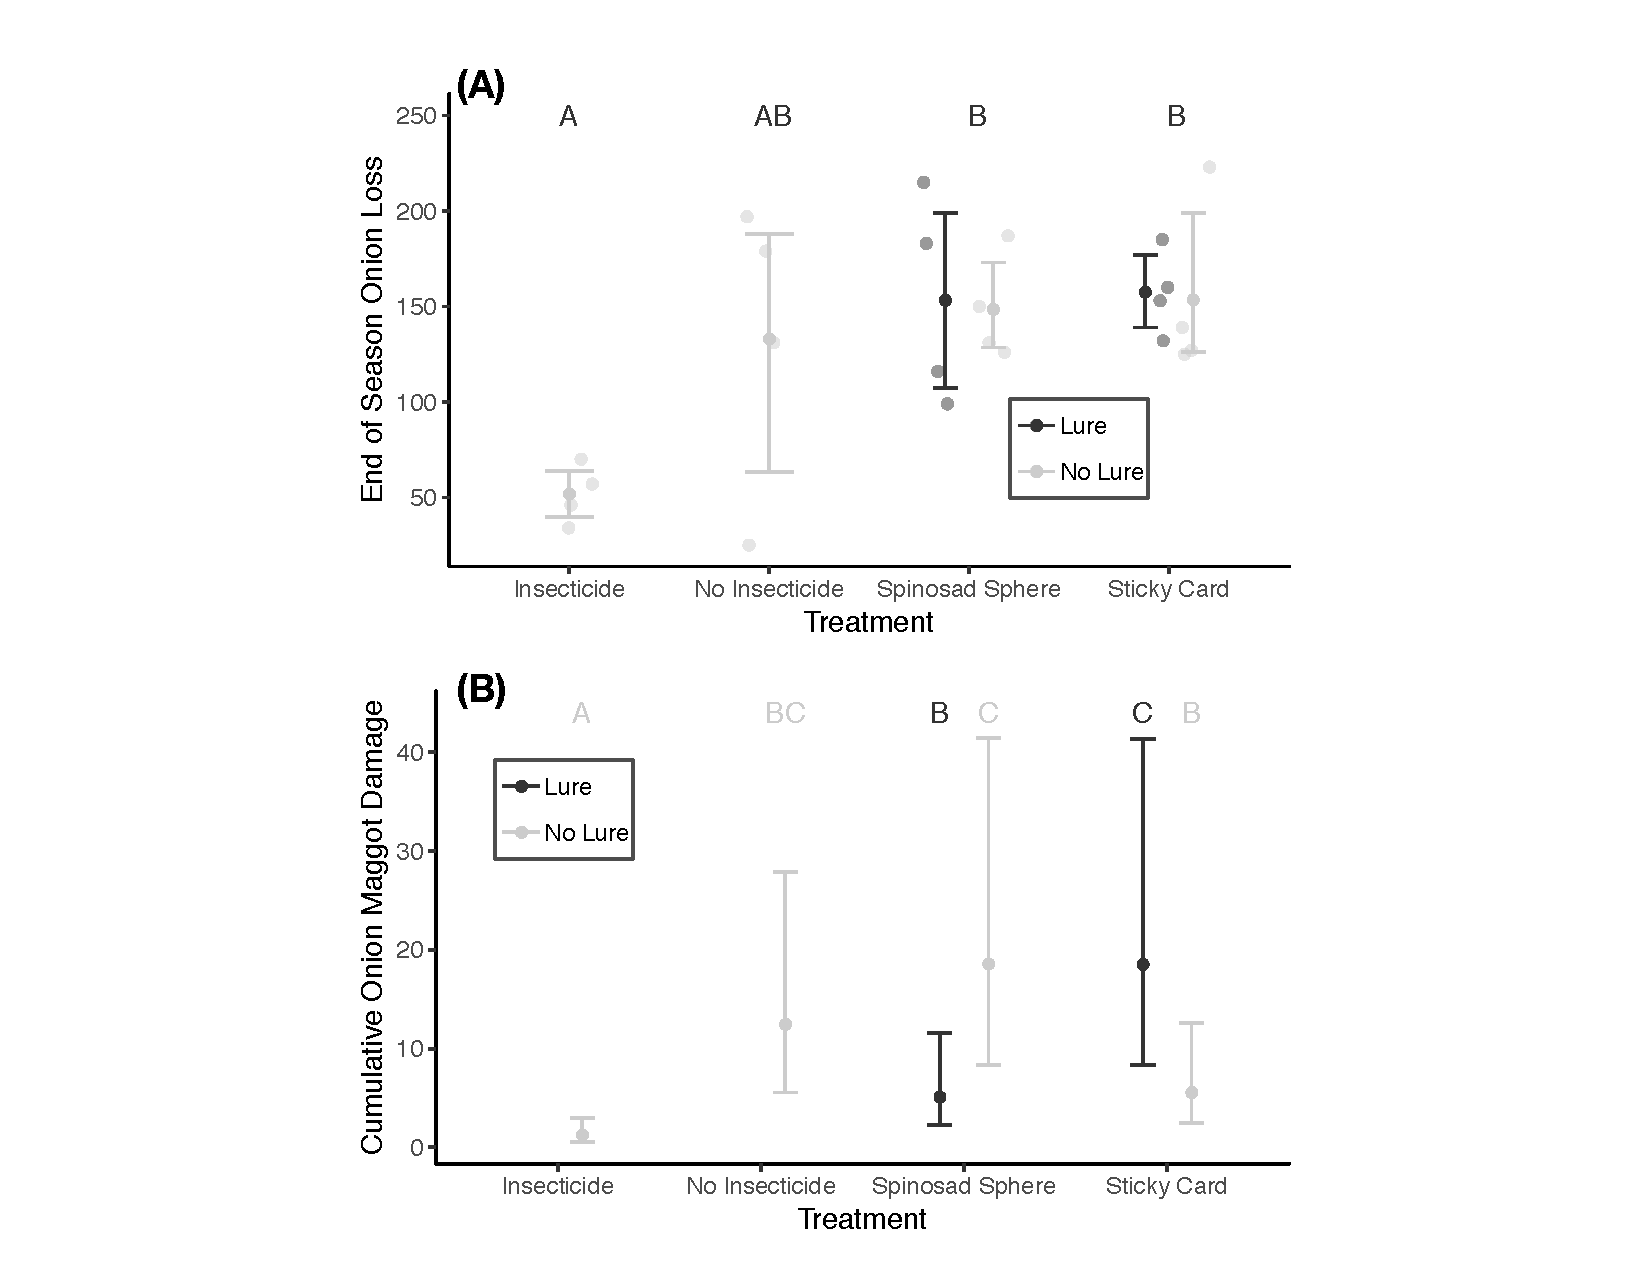
\includegraphics[width = 8cm]{figures/final-figures/figure-4.pdf}
\caption{Field damage of onions.  (A) Cumulative damage (number of dead onion plants) as a result of \textit{D. antiqua} larval feeding.  Solid points and errorbars denote mean effects and 95\% confidence intevals respectively.  Different letters denote significant differences (p \textless 0.05).  (B) Field damage of onion in enclosed cages with differing spinosad sphere formulations.  Cumulative damage is number of dead plants as a result of \textit{D. antiqua} damage.  Points and error bars denote mean and 95\% confidence intervals respectively.  Different letters denote significant differences (p \textless 0.05). } 
\label{fig:figure4}
\end{figure}

\section{Discussion}

Using spinosad containing spheres as an attract and kill solution for control of \textit{D. antiqua} populations may be an effective integrated pest management tool.  Over the course of the three field seasons, with three generations per year (Figure \ref{fig:figure1}), the attract and kill solution was able to consistently inflict mortality on adult \textit{D. antiqua} flies, even after prolonged exposure to field conditions (Figure \ref{fig:figure2}).  While prolonged field exposure did tend to reduce efficacy (Figure \ref{fig:figure2}C) and change the dynamics of mortality (Figure \ref{fig:figure3}), any effects were marginal and may be due to melting (personal observation) of the paraffin solution containing the spinosad (Figure \ref{fig:figure2}D).  

Importantly for practical use of this technique, higher doses of spinosad did not have noticeable effects on \textit{D. antiqua} mortality.  The low rate of spinosad containing spheres resulted in adult \textit{D. antiqua} mortality that was not significantly different than mortality resulting from contact with spheres containing higher levels of spinosad (Figure \ref{fig:figure2}B).  This suggests that inclusion of spinosad as the insecticide component of this attract and kill technique was not only an effective choice for implementation of an attract and kill strategy, but also is a viable option even at low doses.  

The viability of low doses could be particularly important in light of other uses of spinosad in onion fields.  Spinosad seed treatment is a widespread method used for control of onion maggot and common in other commercial seed treatments \citep{nault2006performance,nault2006onion, wilson2015evaluation}.  It is also present in the FI500 seed treatment and alone can offer comparable control \citep{nault2006performance,nault2006onion, wilson2015evaluation}.  These seed treatments are effective options of control of the larval stage; attract and kill methodologies using spinosad evaluated here target the mobile adults.  While exposure to an additional source of spinosad may foster development of resistance, strategies for preventing development of resistance could include rotating use of the active ingredient for the 'kill' part of the attract and kill strategy.   

Numbers of adult \textit{D. antiqua}  killed as a result of the attract and kill strategy using spinosad can be estimated using \textit{D. antiqua} population averages from field experiments and mortality achieved by field-exposed spheres over time assessed in the laboratory.  During peak flights, approximately 272 \textit{D. antiqua} adults (both males and females) were caught by sticky cards on average per week.  Over the course of the field season, approximately 64 adults were caught by sticky cards on average per week.  Assuming spinosad containing spheres kill approximately 54\% of the adults they contact, over the course of a 16 week season, this attract and kill solution could have killed approximately 553 \textit{D. antiqua} adults (16 weeks x 64 adults on average per week * 0.54 mortality) per spinosad containing sphere.  

Comparisons of attract and kill strategies with insecticide and no insecticide controls suggest that spinosad containing spheres are reducing some damage by \textit{D. antiqua} larvae.  Spinosad spheres in conjunction with the attractive Delia Lure resulted in levels of onion damage almost as good as insecticide controls, but with variation that led to overlap with no insecticide negative controls.  In caged field trials, spinosad containing spheres reduced damage resulting from \textit{D. antiqua} feeding to below that of no insecticide controls.  Interestingly, pairing Delia Lure with sticky cards produced higher levels of damage.  This is likely because the kill part of the attract and kill sticky card solution was ineffective; Delia Lure likely attracted adult fly populations to plots but sticky cards did not cause sufficient mortality.  Augmenting spinosad spheres with ammonium carbonate and casein hydrolysate, added to increase longevity of the paraffin,  did not appreciably change control with this attract and kill method.  

While not as effective as insecticide controls, using this attract and kill approach with spinosad spheres may be a choice where other options are not viable or as a complementary tool in an integrated pest management program.  Spinosad spheres do cause adult \textit{D. antiqua} mortality over extended field seasons.  In situations where immediate reduction in damage from \textit{D. antiqua} is desired, this attract and kill approach may be desired in situations where conventional insecticide management is not available either with resistant populations or in organic production systems.  Additionally, this attract and kill approach could be used as a control option where conventional pesticides are no longer effective or available. This strategy could also hold promise as an additional mortality factor in longer term management to control \textit{D. antiqua} populations.  

Efficacy of this attract and kill strategy using spinosad containing spheres to control \textit{D. antiqua} could be enhanced through improving trap placement and density.  \textit{D. antiqua} adults are not uniformly distributed in onion fields, but tend to be found in higher numbers along field edges \citep{werling2006spatial}.  The numbers of the spinosad containing spheres and their placement along edges of commercial onion fields could be adjusted to have a greater impact on increasing fly mortality and reducing maggot damage.  A higher density of spheres in locations where maggot damage is a problem might have a more appreciable impact on reducing damage. Strategic placement of spinosad spheres in areas where populations are highest may further increase efficacy of this technique.  Additionally, increasing sphere density and temporally targeting the first \textit{D. antiqua} generation which causes the most damage, may substantially improve efficacy of this technique and warrant further investigation.  

\section*{Acknowledgements}
We appreciate technical assistance by M. Hessney and Delia Lure contributions from J. Meneley. Starker Wright aided in development and construction of spheres.  The New York State Integrated Pest Management Program, USDA/CSREES Pest Management Alternatives Program, and New York State Department of Agriculture and Markets Onion Research and Development Program supported this research. 

\section*{Conflict of Interest}
The authors declare no conflict of interest.  

\section*{Author Contribution}
BAN, JPN, and SW designed the experiments.  DSW, CCF, and BAN analyzed the data and wrote the manuscript.  


\section*{Data Availability Statement}
All code and data, including manuscript documentation, is available on GitHub(https://github.com/acetworld/onion-maggot-control).

%\printendnotes


\section{References}

\bibliographystyle{vancouver-authoryear}
\bibliography{om-attraction}

%\graphicalabstract{example-image-1x1}{Please check the journal's author guildines for whether a graphical abstract, key points, new findings, or other items are required for display in the Table of Contents.}

\end{document}
